\documentclass[10pt, en-GB]{beamer}

\usetheme[numbering = fraction, progressbar = frametitle,]{metropolis}
\usepackage{appendixnumberbeamer}
\usepackage{bbm}

\usepackage{booktabs}
\usepackage[scale=2]{ccicons}
\usepackage{multirow,array}
\usepackage{datetime2}
\usepackage{appendixnumberbeamer}
\DTMsetup{useregional=numeric}
\DTMtryregional{en}{GB}

\usepackage{pgfplots}
\usepgfplotslibrary{dateplot}

\usepackage{xspace}
\newcommand{\themename}{\textbf{\textsc{metropolis}}\xspace}
\renewcommand{\Pr}{\mathbbm{P}}

\setbeamertemplate{frame footer}{Eggers \& Nowacki (2019)}

\title{Comparing Strategic Voting Incentives in Plurality and Instant-Runoff Elections}
\subtitle{}
\date{\today}
\author{Andy Eggers (Nuffield College, Oxford) \\ Toby Nowacki (Stanford)}
% \titlegraphic{\hfill\includegraphics[height=1.5cm]{logo.pdf}}

\begin{document}

\maketitle

\metroset{block=fill}

% \begin{frame}{Table of contents}
%   \setbeamertemplate{section in toc}[sections numbered]
%   \tableofcontents[hideallsubsections]
% \end{frame}

\begin{frame}[t]\frametitle{Introduction}
    \begin{itemize}[<+->]
    	\item Sometimes you can be better off by misrepresenting your true preferences in order to obtain a better outcome overall: you have an incentive to \textbf{vote strategically}.
    	\begin{itemize}
    		\item {\color{gray} In 2000, Nader voters in Fla. had an incentive to vote for Gore instead}
    	\end{itemize}
    	\item No electoral system is immune to strategic incentives. (Sattherthwaite 1975)
    	\item How likely are these strategic incentives in the real world, with observed beliefs and preferences?
    	\item Better educated citizens are more likely to act on their strategic incentives $\Rightarrow$ advantage in systems that strongly incentivise strategic voting
    	\begin{itemize}
    		\item {\color{gray} also make results more difficult to interpret and impose additional costs on voters}
    	\end{itemize}
    \end{itemize}
\end{frame}

\begin{frame}[t]\frametitle{Introduction: Plurality and IRV}
    \begin{itemize}[<+->]
    \item Our focus is on two voting systems: plurality (FPTP) and IRV (ranked choice voting, alternative vote, ...)
    \item In \textbf{plurality}, voters cast a ballot for one candidate.
    \begin{itemize}
    	\item The candidate with the most ballots wins.
    \end{itemize}
    \item In \textbf{IRV}, voters rank all candidates. 
    \begin{itemize}
    	\item The candidate with the fewest first-ranked ballots is eliminated, and her votes redistributed according to the second rank.
    	\item This is repeated until a candidate has obtained a majority of votes.
    \end{itemize}
    \item `Folk' conjectures that strategic voting is less beneficial under IRV than under Plurality (e.g., UK 2011 referendum)
    \item \textbf{This paper:} how do strategic incentives look like under either system, both qualitatively and quantitatively?
    \end{itemize}
    \hyperlink{strat_qual}{\beamerbutton{Types of strategic votes in electoral systems}}
\end{frame}

\begin{frame}[t]\frametitle{General Framework}

\alert{Set-up.} Let there be $K$ candidates, $B$ admissible ballot types (e.g., in Plurality, $b = 3$), and $N$ voters.

\alert{Probability of winning.} Let $\bf P$ denote a $K \times B$ matrix where each column is a vector of candidates' winning probability as a function of an additional ballot $b$.

\alert{Voters' utility.} Let $\bf U$ denote a $N \times K$ matrix where each row is a vector of any voter's utilities from a given candidate winning.

\alert{Expected utility from any ballot type.} Finally, let $\bf \bar{U} = UP$ denote the expected utility from each ballot type for any voter.


\end{frame}

\begin{frame}[t]\frametitle{General Framework (cont'd)}

\alert{Strategic voting.} For every voter $i$, the strategic voting incentive is defined as:

\begin{equation}
	\text{Expected Benefit} = \text{arg } \underset{b}{\text{max }} {\bf \bar{u}}(b) - {\bf \bar{u}}(b_s)
\end{equation}

where $\bf \bar{u}$ is the $i$th row from the expected utility matrix $\bf \bar{U} = UP$.

\pause
\begin{block}{Example}
\begin{equation*}
	{\bf \bar{u}}_{\text{Plur}} = \begin{bmatrix}
	\textbf{0.67} & 0.57 & 0.33
	\end{bmatrix}
\end{equation*}
\begin{equation*}
	{\bf \bar{u}}_{{IRV}} = \begin{bmatrix}
	0.67 & 0.57 & 0.33 & \textbf{0.86} & 0.21 & 0.40
	\end{bmatrix}
\end{equation*}
\end{block}

\pause
How to model utilities and beliefs / outcome probabilities?

\end{frame}

\begin{frame}[t]\frametitle{Modelling preferences and beliefs}

We rely on CSES data to characterise preferences and beliefs -- election surveys from 160 cases (58 countries). We focus on the three largest parties in every reported survey.
\pause
\begin{block}{Preferences}
	Respondents' party like-dislike scores (on a scale from 0 to 10)
\end{block}
\pause
\begin{block}{Beliefs}
	Given reported preferences in survey, model election outcome beliefs using Dirichlet distribution:

	\begin{equation*}
		f({\bf v}) = \text{Dir} (s \times {\bf v}_0)
	\end{equation*}
\end{block}
\end{frame}

\begin{frame}[t]\frametitle{Modelling preferences and beliefs (cont'd)}

\begin{block}{Beliefs (cont'd)}
\begin{itemize}
\item Expected outcome (mode of distribution): vote shares if everyone in survey voted sincerely $\Rightarrow$ iterative polling algorithm to adjust for `strategicness'.
\item Precision parameter: using previous empirical work, between $s = 10$ and $s = 85$. 
\item Given the distribution over election outcomes, we can also specify the probabilities of each candidate winning for each type of marginal ballot.
\end{itemize} 
\end{block}    
\end{frame}


\begin{frame}[t]\frametitle{Iterative polling algorithm}
    
\begin{itemize}[<+->]
	\item It might seem unreasonable for voters to expect that everyone else votes sincerely -- equally they may not anticipate a full strategic equilibrium.
	\item We `simulate' a series of polls for each survey case, starting with the sincere profile: 
		\begin{itemize}
			\item Give voters a poll of everyone's sincere preference and assume that a proportion $\lambda$ will best-respond by voting strategically
			\item Pass new poll with proportion $\lambda$ of best-responders and everyone else still voting sincerely to everyone and calculate new best response
			\item Iterate until fixed point reached: best responses no longer change in light of polling information.
		\end{itemize}
	\item We compute strategic voting incentives `along the path' -- checking for different assumptions about voters' strategicness.
	\item For empirics, we set $\lambda = .05$.
\end{itemize}

\end{frame}

\begin{frame}[t]\frametitle{Results: Iterative polling algorithm}
    
\begin{figure}
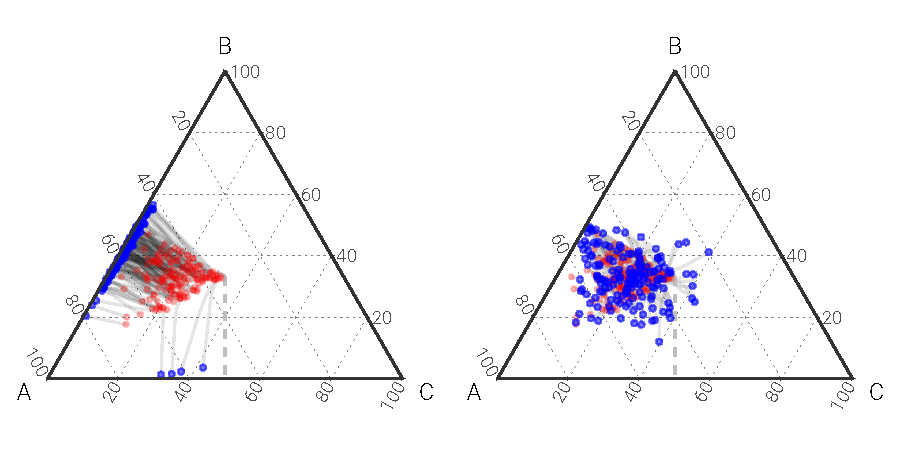
\includegraphics[width = 0.9\textwidth]{pres_fig/tatonnement_both}
\caption{Iterative polling paths in Plurality (left) and IRV (right). Red dots mark sincere profiles, blue dots mark ballot distribution after 60 iterations.}
\end{figure}

\end{frame}

\begin{frame}[t]\frametitle{Results: Expected benefit of strategic voting}
    
\begin{figure}
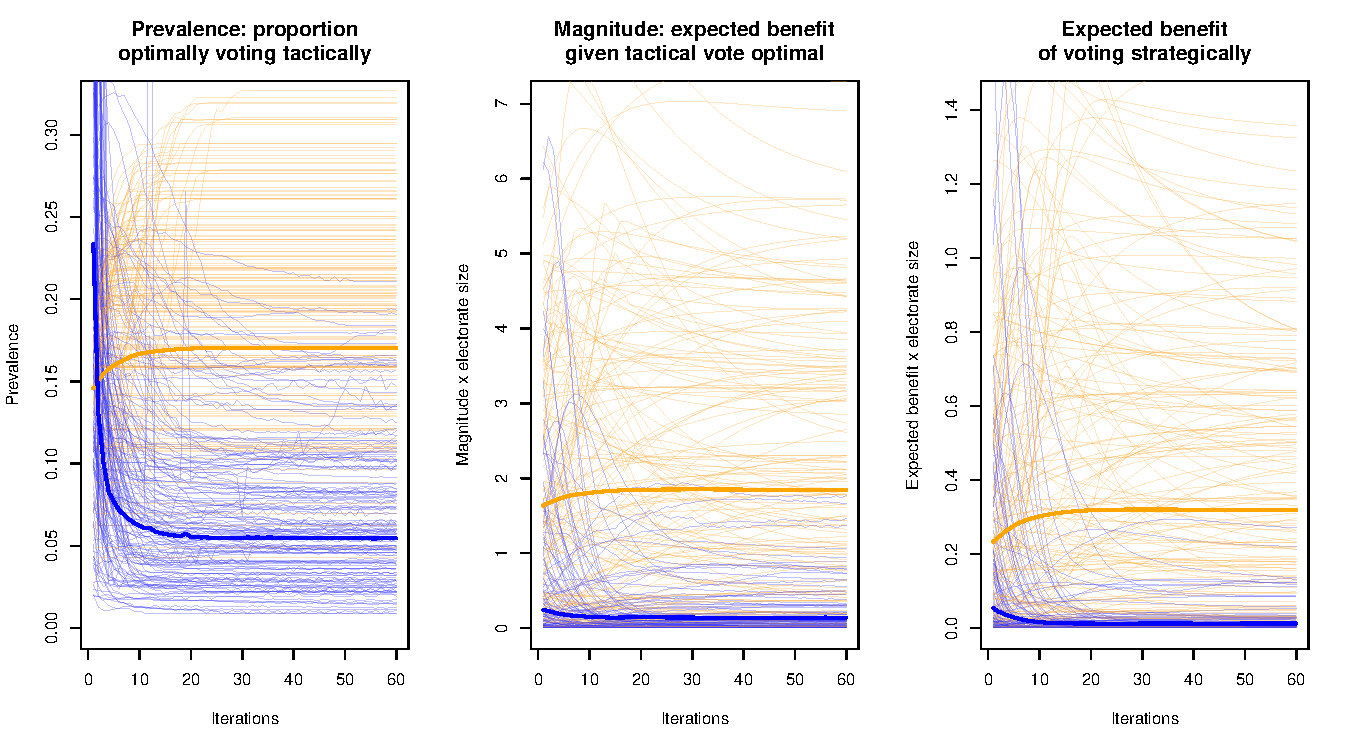
\includegraphics[width = .9\textwidth]{pres_fig/results_85} 
\caption{Main results: Prevalence, Magnitude, and Expected Benefit of strategic voting in Plurality (orange) and IRV (blue) for a precision parameter of $s = 85$, where $\text{Prevalence $\times$ Magnitude} = \text{Expected Benefit}$ [intensive / extensive margin].}
\end{figure}
\end{frame}

\begin{frame}[t]\frametitle{Discussion}
    
\begin{alertblock}{Key results}
\begin{itemize}[<+->]
\item Expected benefit is significantly higher in Plurality (by factor of 5 - 30)
\item For the most part, both magnitude and prevalence of strategic incentives are also higher in Plurality
\item Only when others are expected to vote sincerely, and belief precision is high, is there high prevalence of strategic voting incentives in IRV (but still with low magnitude)
\end{itemize}
\end{alertblock}

Partial explanations:
\begin{itemize}[<+->]
	\item events that reward strategic vote in IRV are less likely
	\item strategic voting more likely to backfire in IRV (risk of electing least favoured candidate)
	\item strategic incentives can be "substitutes" in IRV
\end{itemize}
\hyperlink{disc}{\beamerbutton{Jump}}

\end{frame}

\appendix

\section{Qualitative description of strategic voting in Plurality and IRV (h/t Andy)}
\label{strat_qual}

\begin{frame}{Strategic voting in FPTP} 

Given candidates $\{a, b, c\}$, three possible ballots: $\{a, b, c\}$.\\ \bigskip \pause 

Three ways to affect outcome: \bigskip %  $ab$ tie for first, $ac$ tie, $bc$ tie.  \\ \bigskip \pause 

\begin{minipage}{.33\textwidth}
\centering $ab$ tie \\ 
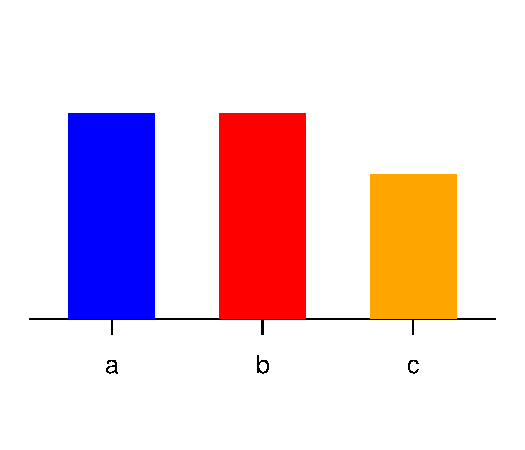
\includegraphics[width=\textwidth]{pres_fig/cases_for_paper/plurality_ties_for_first_1.pdf}
\end{minipage}%
\begin{minipage}{.33\textwidth}
\centering $ac$ tie \\ 
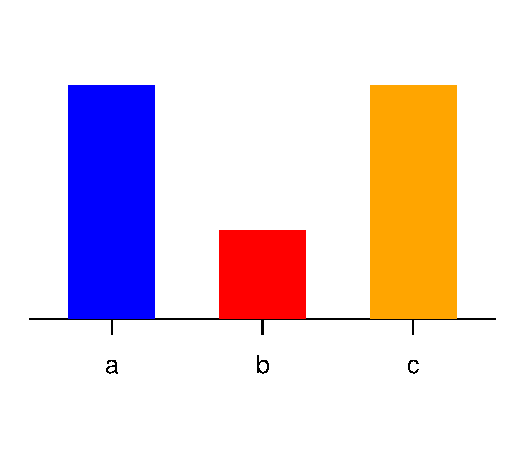
\includegraphics[width=\textwidth]{pres_fig/cases_for_paper/plurality_ties_for_first_2.pdf}
\end{minipage}%
\begin{minipage}{.33\textwidth}
\centering $bc$ tie \\ 
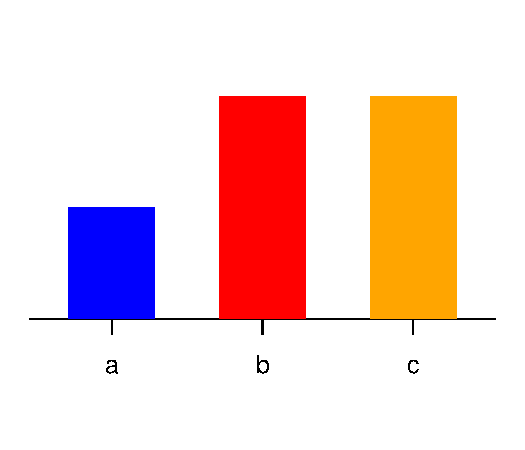
\includegraphics[width=\textwidth]{pres_fig/cases_for_paper/plurality_ties_for_first_3.pdf}
\end{minipage}

\pause 

\textbf{Strategic logic:} ``Desert a trailing candidate to avoid wasting one's vote.''  \\
\end{frame} 




\begin{frame}{Strategic voting in IRV} 

Six possible ballots: $\{abc, acb, bac, bca, cab, cba\}$. \\ \bigskip \pause 

Twelve ways to affect outcome: 

\begin{itemize}
\item determine who is eliminated, thereby determining winner \textcolor{gray}{(9 ways)}
\item determine who wins post-elimination \textcolor{gray}{(3 ways)} 
\end{itemize} 

\pause \bigskip 
%Similar to  runoff \textcolor{gray}{(e.g.\ French pres.)}, but
%\begin{itemize}
%\item no incentive to secure victory in ``first round''
%\item ``second-round'' vote constrained by ``first round'' 
%\end{itemize}  

Two types of \textbf{strategic logic in IRV}: 
\begin{enumerate} 
\item ``Desert a leading candidate to avoid wasting one's vote''
	\begin{itemize}
		\item Center-left voter: `Macron will advance, so I'll rank Fillon/Le Pen first'
	\end{itemize}     \pause 
\item ``Desert a trailing candidate to avoid electing one's least favorite''
	\begin{itemize}
		\item Right-wing voter: `Le Pen can't beat Macron, so I'll rank Fillon first'
	\end{itemize} 
\end{enumerate} 

% complicated 
% interactions important. 
\end{frame} 

\begin{frame}{Positive feedback in FPTP elections}

\begin{center}
\begin{minipage}{0.45\textwidth} 
\begin{center}
\includegraphics<1->[height=0.8\textheight]{pres_fig/cases_for_paper/barplot_case_4_1.pdf}
\end{center} 

\vspace{-.5in} 
\onslide<2->{\scriptsize{Discrepancy in support for $c$ vs.\ other candidates $\implies$ $c \rightarrow a$, $c \rightarrow b$ votes.}}

\end{minipage}% 
\begin{minipage}{0.1\textwidth}
\textcolor{white}{Hidden} 
\end{minipage}% 
\begin{minipage}{0.45\textwidth} 

\begin{center}
\includegraphics<3->[height=0.8\textheight]{pres_fig/cases_for_paper/barplot_case_4sv_1.pdf}
\end{center}

\vspace{-.5in} 
% \onslide<3->{\scriptsize{\textcolor{white}{Discrepancy between $b$'s and $c$'s 2nd prefs $\implies$ $acb \rightarrow cab$, $abc \rightarrow cab$, $cba \rightarrow bca$ votes.}}}
\onslide<4->{\scriptsize{\textcolor{black}{Strategic responses to discrepancy  $\implies$ \textcolor{white}{hid} discrepancy widens.}}}

\end{minipage} 
\end{center}
\end{frame} 





\begin{frame}{Negative feedback in IRV elections}

\begin{center}
\begin{minipage}{0.45\textwidth} 
\begin{center}
\includegraphics<1>[height=0.8\textheight]{pres_fig/cases_for_paper/barplot_case_3_1.pdf}
\includegraphics<2->[height=0.8\textheight]{pres_fig/cases_for_paper/barplot_case_3_2.pdf}
\end{center} 

\vspace{-.5in} 
\onslide<3->{\scriptsize{Discrepancy btw $b$'s and $c$'s 2nd prefs $\implies$ $acb \rightarrow cab$, $abc \rightarrow cab$, $cba \rightarrow bca$ votes.}}

\end{minipage}% 
\begin{minipage}{0.1\textwidth}
\textcolor{white}{Hidden} 
\end{minipage}% 
\begin{minipage}{0.45\textwidth} 

\begin{center}
\includegraphics<4>[height=0.8\textheight]{pres_fig/cases_for_paper/barplot_case_3sv_1.pdf}
\includegraphics<5->[height=0.8\textheight]{pres_fig/cases_for_paper/barplot_case_3sv_2.pdf}
\end{center}

\vspace{-.5in} 
% \onslide<3->{\scriptsize{\textcolor{white}{Discrepancy between $b$'s and $c$'s 2nd prefs $\implies$ $acb \rightarrow cab$, $abc \rightarrow cab$, $cba \rightarrow bca$ votes.}}}
\onslide<6->{\scriptsize{\textcolor{black}{Strategic responses to discrepancy  $\implies$ \textcolor{white}{hid} discrepancy narrows.}}}

\end{minipage} 
\end{center}
\end{frame} 


\section{Further discussion of results}
\label{disc}

\begin{frame}[t]\frametitle{Likelihood of `pivotal events'}
    
\emph{Events that reward strategic votes in IRV are less likely}


\begin{columns}[T] % align columns
\begin{column}{.48\textwidth}
\begin{itemize}
	\item In Plurality, we need a tie (close result) between the first and and the second candidate.
	\item In IRV, two candidates must tie in first preferences \textbf{and} we need a tie (close result) in second preferences in the run-off.
\end{itemize}
\end{column}%
\hfill%
\begin{column}{.48\textwidth}
\begin{figure}[tb]
	\centering
	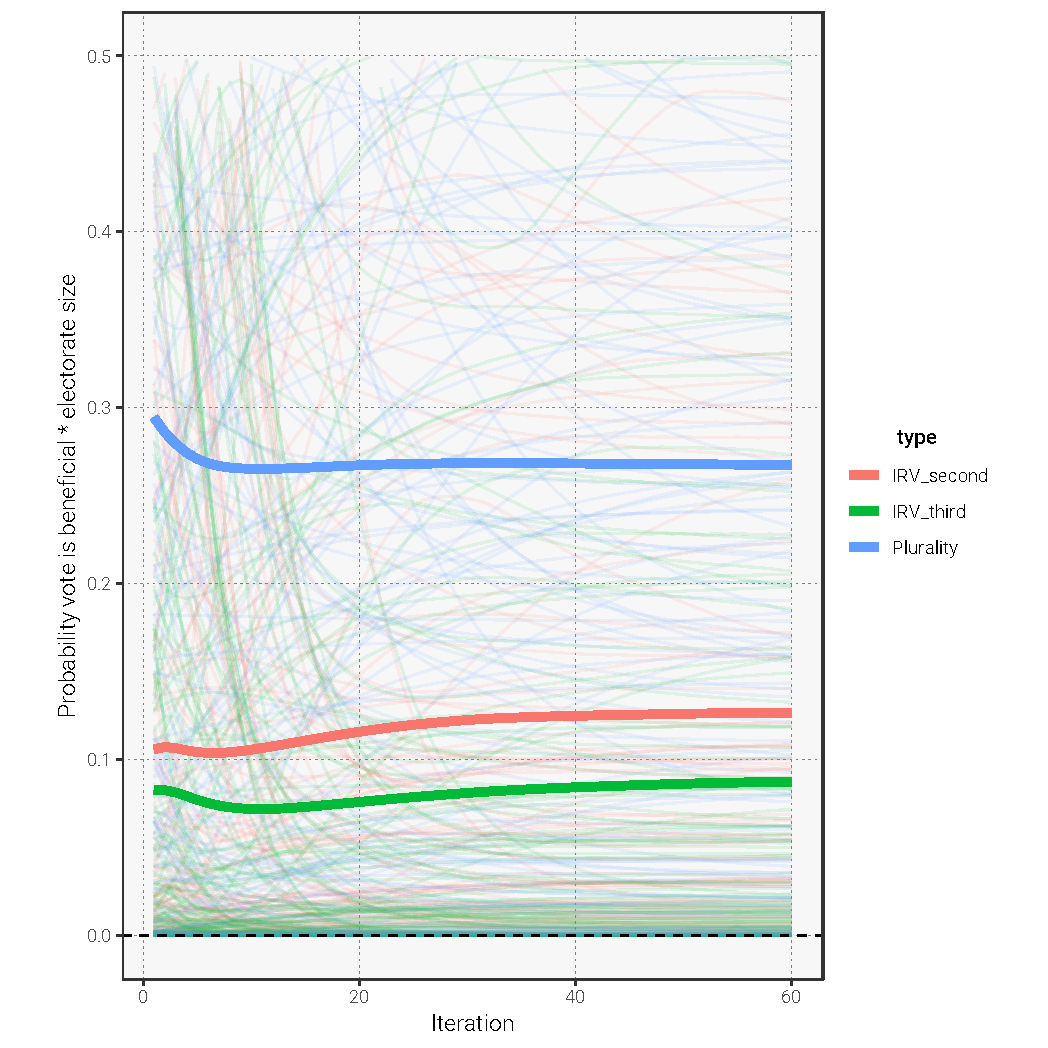
\includegraphics[width = \textwidth]{pres_fig/conj1.pdf}
	\caption{Expected probability of strategic vote being beneficial (weighted by electorate size)}
	\label{fig:conj1}
\end{figure}

\end{column}%
\end{columns}

\end{frame}

\begin{frame}[t]\frametitle{Conflicting events}
    
\emph{Strategic voting in IRV is more likely to backfire}


\begin{columns}[T] % align columns
\begin{column}{.48\textwidth}
\begin{itemize}
	\item In \textbf{Plurality}, only first/second tied: deserted third can be far away
	\item For strategic voting in \textbf{IRV} to be beneficial, all three candidates must be reasonably close to one another -- greater risk of backfiring!

\end{itemize}
\end{column}%
\hfill%
\begin{column}{.48\textwidth}
\begin{figure}[tb]
	\centering
	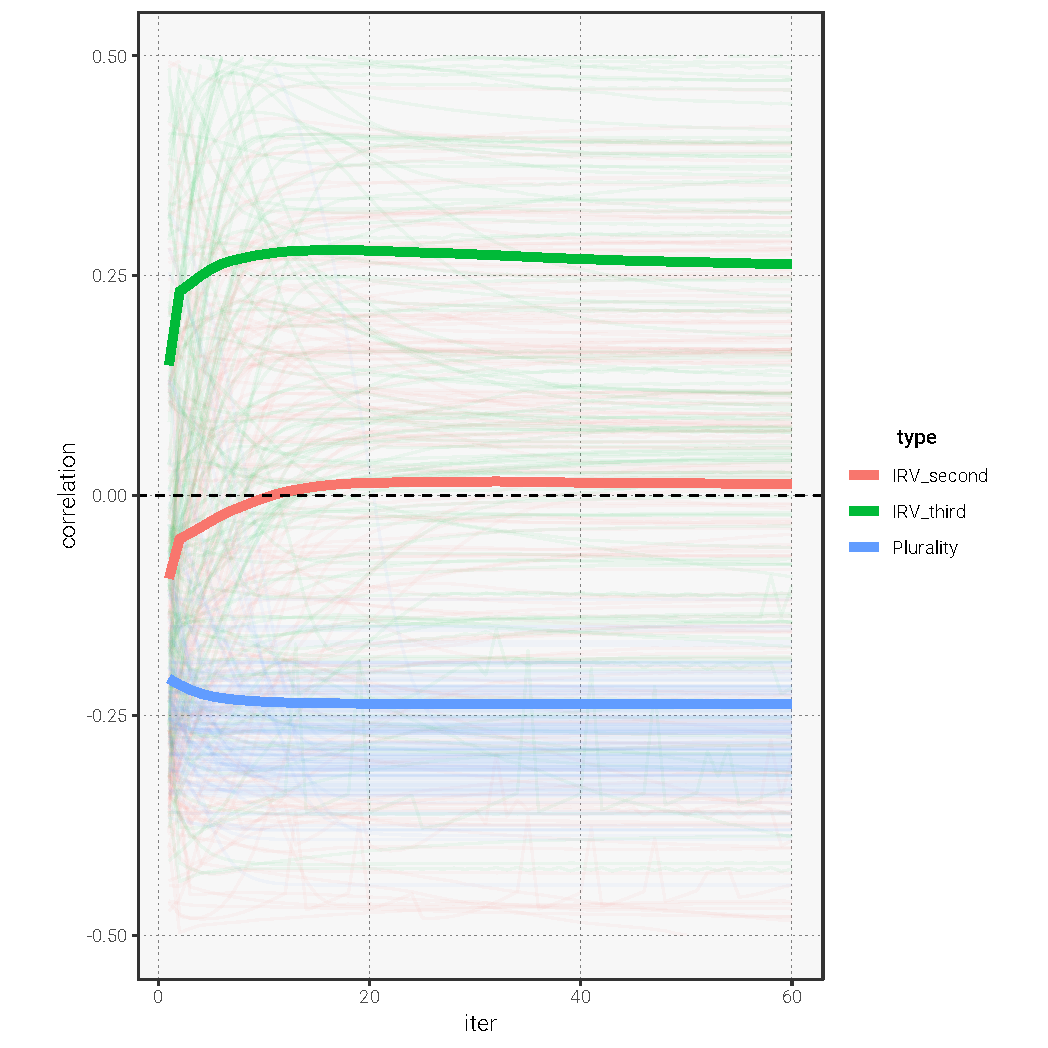
\includegraphics[width = \textwidth]{pres_fig/conj2.pdf}
	\caption{Correlation between costs and benefits of strategic vote}
	\label{fig:conj2}
\end{figure}

\end{column}%
\end{columns}

\end{frame}

\begin{frame}[t]\frametitle{Conflicting events}
    
\emph{Strategic voting in IRV is characterised by substitutes}

\begin{itemize}
	\item In \textbf{Plurality}, if others desert the third-placed candidate, my incentive to do so, too, grows ($C$ less likely to win overall)
	\item In \textbf{IRV}, if other $CBA$ voters vote $ACB$, my incentive to do so, too, diminishes: risk of accidentally electing $A$ increases (when $A$ beats $C$ in second round)

\end{itemize}

\end{frame}




\end{document}
